\section{Research chapters}

The account of the scholarly work should be presented in a manner suitable for the field. It should be complete, systematic, and sufficiently detailed to enable a reader to understand how the data were gathered and analyzed, and how to apply similar methods in another study. Notation and formatting must be consistent throughout the thesis, including units of measure, abbreviations, and the numbering scheme for tables, figures, footnotes, and citations. One or more chapters may consist of material published (or submitted for publication) elsewhere, or other artifacts (e.g., film, application-oriented documents) placed in a scholarly context. See “Including Published Material in a Thesis or Dissertation” for additional details.

\subsection{Data}

% Example of a table:
\begin{table}[H]
\caption{Sample information}
\label{table:sampleinfo}
\vspace{-.5em}
\begin{tabularx}{\textwidth}{@{}YYY@{}}
\rowcolor{tableheader}
Sample ID & Category & Status \\
one & A & Healthy \\
two & B & Sick \\
\end{tabularx}
\end{table}

\subsection{Methods}
\subsubsection{Method 1}
\subsubsection{Method 2}
\subsection{Results}
\subsubsection{Result 1}

% Example of a figure:
\begin{figure}[H]
  \centering
  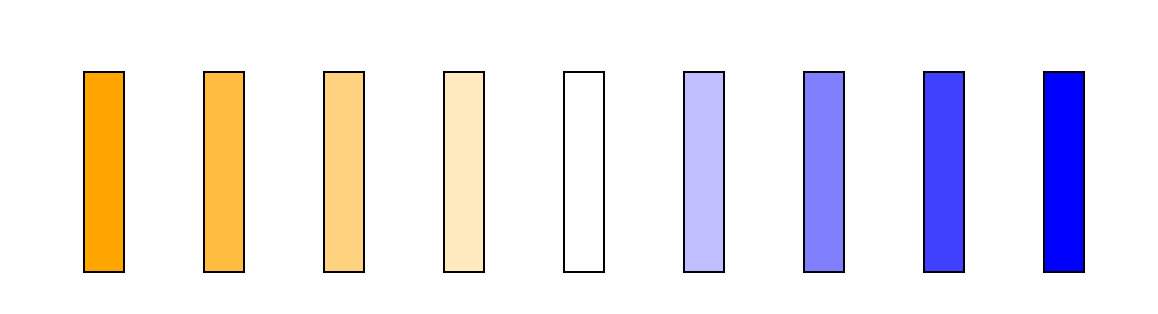
\includegraphics[width=0.75\textwidth]{figures/fig1.png}
  \vspace{-.5em}
  \caption{\nbars~bars}
  \label{fig:fig1}
\end{figure}

\subsubsection{Result 2}

% Example of using references to the lablel:
In Figure~\ref{fig:fig1}, we show a spectrum with \nbars~bars.
In Table~\ref{table:sampleinfo}, we have a 3 by 3 table.
